\documentclass[tikz,border=4]{standalone}\usepackage[]{graphicx}\usepackage[]{xcolor}
% maxwidth is the original width if it is less than linewidth
% otherwise use linewidth (to make sure the graphics do not exceed the margin)
\makeatletter
\def\maxwidth{ %
  \ifdim\Gin@nat@width>\linewidth
    \linewidth
  \else
    \Gin@nat@width
  \fi
}
\makeatother

\definecolor{fgcolor}{rgb}{0.345, 0.345, 0.345}
\newcommand{\hlnum}[1]{\textcolor[rgb]{0.686,0.059,0.569}{#1}}%
\newcommand{\hlsng}[1]{\textcolor[rgb]{0.192,0.494,0.8}{#1}}%
\newcommand{\hlcom}[1]{\textcolor[rgb]{0.678,0.584,0.686}{\textit{#1}}}%
\newcommand{\hlopt}[1]{\textcolor[rgb]{0,0,0}{#1}}%
\newcommand{\hldef}[1]{\textcolor[rgb]{0.345,0.345,0.345}{#1}}%
\newcommand{\hlkwa}[1]{\textcolor[rgb]{0.161,0.373,0.58}{\textbf{#1}}}%
\newcommand{\hlkwb}[1]{\textcolor[rgb]{0.69,0.353,0.396}{#1}}%
\newcommand{\hlkwc}[1]{\textcolor[rgb]{0.333,0.667,0.333}{#1}}%
\newcommand{\hlkwd}[1]{\textcolor[rgb]{0.737,0.353,0.396}{\textbf{#1}}}%
\let\hlipl\hlkwb

\usepackage{framed}
\makeatletter
\newenvironment{kframe}{%
 \def\at@end@of@kframe{}%
 \ifinner\ifhmode%
  \def\at@end@of@kframe{\end{minipage}}%
  \begin{minipage}{\columnwidth}%
 \fi\fi%
 \def\FrameCommand##1{\hskip\@totalleftmargin \hskip-\fboxsep
 \colorbox{shadecolor}{##1}\hskip-\fboxsep
     % There is no \\@totalrightmargin, so:
     \hskip-\linewidth \hskip-\@totalleftmargin \hskip\columnwidth}%
 \MakeFramed {\advance\hsize-\width
   \@totalleftmargin\z@ \linewidth\hsize
   \@setminipage}}%
 {\par\unskip\endMakeFramed%
 \at@end@of@kframe}
\makeatother

\definecolor{shadecolor}{rgb}{.97, .97, .97}
\definecolor{messagecolor}{rgb}{0, 0, 0}
\definecolor{warningcolor}{rgb}{1, 0, 1}
\definecolor{errorcolor}{rgb}{1, 0, 0}
\newenvironment{knitrout}{}{} % an empty environment to be redefined in TeX

\usepackage{alltt}\usepackage{siunitx}
\usetikzlibrary{positioning}
\tikzset{mynode/.style={draw,text width=2 in,align=center}
}
\IfFileExists{upquote.sty}{\usepackage{upquote}}{}
\begin{document}
  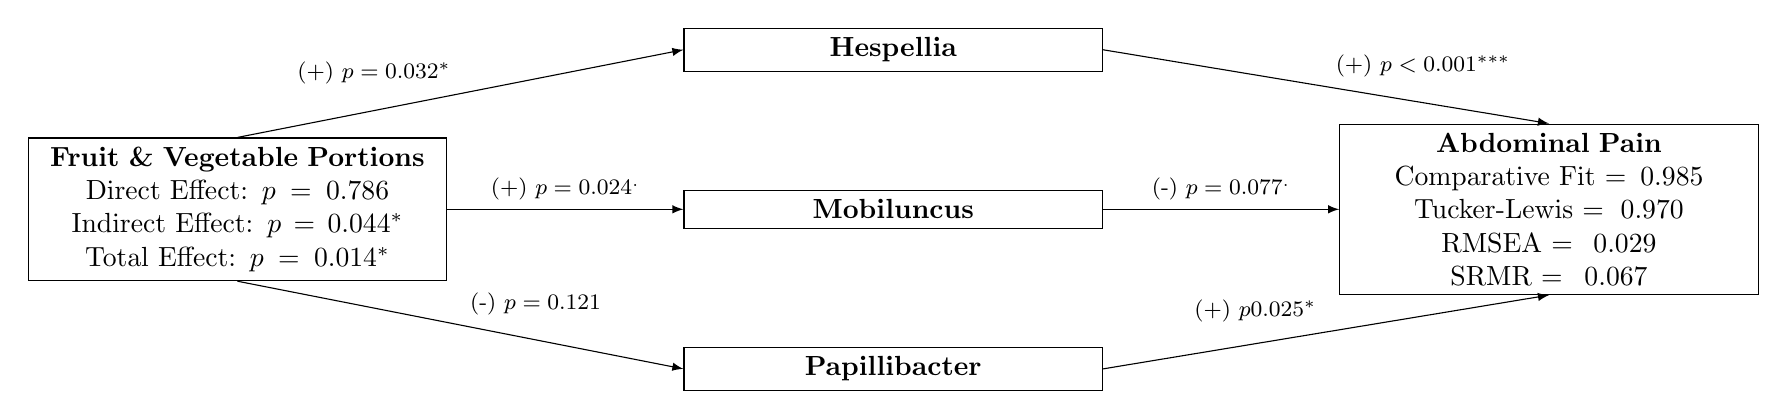
\begin{tikzpicture}
  
  % Mediators
    \node[mynode] (m1){\textbf{Hespellia}};
    \node[mynode, below = 1.5 of m1] (m2){\textbf{Mobiluncus}};
    \node[mynode, below = 1.5 of m2] (m3){\textbf{Papillibacter}};
    
    % Treatments
    \node[mynode, left = 3 of m2](a) {\textbf{Fruit \& Vegetable Portions} \\ Direct Effect: $p = 0.786$ \\ Indirect Effect: $p = 0.044^{*}$ \\ Total Effect: $p = 0.014^{*}$};
    
    % Health Outcomes
    \node[mynode, right = 3 of m2](b) {\textbf{Abdominal Pain} \\ Comparative Fit $= 0.985$ \\ Tucker-Lewis $= 0.970$ \\ RMSEA $=0.029$ \\ SRMR $=0.067$};
    
    % Fruit to mediators
    \draw[-latex] (a.north) -- node[auto,font=\footnotesize] {(+) $p = 0.032^{*}$} (m1.west);
    \draw[-latex] (a.east) -- node[auto,font=\footnotesize] {(+) $p = 0.024^{.}$} (m2.west);
    \draw[-latex] (a.south) -- node[auto,font=\footnotesize] {(-) $p = 0.121$} (m3.west);
    
    
    % Mediators to outcome
    \draw[-latex] (m1.east) -- node[auto,font=\footnotesize] {(+) $p < 0.001^{***}$} (b.north);
    \draw[-latex] (m2.east) -- node[auto,font=\footnotesize] {(-) $p = 0.077^{.}$} (b.west);
    \draw[-latex] (m3.east) -- node[auto,font=\footnotesize] {(+) $p 0.025^{*}$} (b.south);
    
    

  \end{tikzpicture}
\end{document}
